% Algebra 2 Lesson 3-2 fast-track packet: Adding, Subtracting, and Multiplying Polynomials
% (enVision A2 2024 TE, Example 1 and Example 2 only; draft 2026-10-30, PLC has not met on this lesson)
% Shared preamble for the "fast" (hacked-down) Algebra 2 lesson packets, Oct 2026.
% Each packet: % Shared preamble for the "fast" (hacked-down) Algebra 2 lesson packets, Oct 2026.
% Each packet: % Shared preamble for the "fast" (hacked-down) Algebra 2 lesson packets, Oct 2026.
% Each packet: \input{fast-packet-template} then \begin{document} ... \end{document}.
\documentclass[12pt]{article}
\usepackage[margin=0.7in]{geometry}
\usepackage{amsmath,amssymb}
\usepackage{booktabs,tabularx,array}
\usepackage{enumitem}
\usepackage[T1]{fontenc}
\usepackage[utf8]{inputenc}
\usepackage{lmodern}
\usepackage{tikz}
\usepackage{pgfplots}
\pgfplotsset{compat=1.18}
\usepackage{xcolor}
\setlist{nosep,leftmargin=1.4em}
\setlength{\parindent}{0pt}
\setlength{\parskip}{6pt}
\renewcommand{\arraystretch}{1.35}
\newcolumntype{Y}{>{\raggedright\arraybackslash}X}
\pagestyle{empty}

% blanks and workspace
\newcommand{\blank}[1][2.6cm]{\rule[-2pt]{#1}{0.5pt}}
\newcommand{\lines}[1][1]{\par\vspace{2pt}\foreach \i in {1,...,#1}{\rule{0pt}{22pt}\rule{\linewidth}{0.4pt}\par}}
\newcommand{\wspart}[2]{\vspace{4pt}{\large\bfseries #1: #2}\par\vspace{-6pt}\rule{\textwidth}{0.4pt}\par}

% header: \packethead{Lesson 1-3}{Piecewise-Defined Functions}
\newcommand{\packethead}[2]{%
{\LARGE\bfseries #2}\hfill Name \blank[5cm]\\[2pt]
Algebra 2 \quad #1 (fast track) \hfill Date \blank[2.5cm] \quad Period \blank[1.2cm]\par\vspace{2pt}}

% boxed goals: \goals{learning goal}{language goal}
\newcommand{\goals}[2]{%
\fbox{\parbox{\dimexpr\textwidth-2\fboxsep-2\fboxrule}{%
\textbf{Learning goal:} #1\\[2pt]
\textbf{Language goal:} #2}}\par}

% quiz target box: \quiztarget{text}
\newcommand{\quiztarget}[1]{%
\vspace{4pt}\colorbox{gray!12}{\parbox{\dimexpr\textwidth-2\fboxsep}{\textbf{On the quiz:} #1}}\par}

% IXL table row helper: code & skill & which quiz question it feeds
\newcommand{\ixlrow}[3]{\texttt{#1} & #2 & #3 \\}

% one grid style for every graph; override xmin/xmax/... per plot
\pgfplotsset{sheetgrid/.style={
  axis lines=middle, grid=both, grid style={gray!45},
  xmin=-10.5, xmax=10.5, ymin=-10.5, ymax=10.5,
  xtick={-10,-8,...,10}, ytick={-10,-8,...,10},
  x=0.28cm, y=0.28cm,
  ticklabel style={font=\scriptsize, fill=white, inner sep=1pt},
  xlabel={$x$}, ylabel={$y$},
  axis line style={thick}, clip=true}}
% unit grid for small windows
\pgfplotsset{unitgrid/.style={sheetgrid,
  xmin=-5.5, xmax=5.5, ymin=-5.5, ymax=5.5,
  xtick={-5,...,5}, ytick={-5,...,5}, x=0.5cm, y=0.5cm}}
% open and closed endpoints
\tikzset{closed/.style={circle, fill, inner sep=1.6pt},
         open/.style={circle, draw, fill=white, inner sep=1.4pt}}
 then \begin{document} ... \end{document}.
\documentclass[12pt]{article}
\usepackage[margin=0.7in]{geometry}
\usepackage{amsmath,amssymb}
\usepackage{booktabs,tabularx,array}
\usepackage{enumitem}
\usepackage[T1]{fontenc}
\usepackage[utf8]{inputenc}
\usepackage{lmodern}
\usepackage{tikz}
\usepackage{pgfplots}
\pgfplotsset{compat=1.18}
\usepackage{xcolor}
\setlist{nosep,leftmargin=1.4em}
\setlength{\parindent}{0pt}
\setlength{\parskip}{6pt}
\renewcommand{\arraystretch}{1.35}
\newcolumntype{Y}{>{\raggedright\arraybackslash}X}
\pagestyle{empty}

% blanks and workspace
\newcommand{\blank}[1][2.6cm]{\rule[-2pt]{#1}{0.5pt}}
\newcommand{\lines}[1][1]{\par\vspace{2pt}\foreach \i in {1,...,#1}{\rule{0pt}{22pt}\rule{\linewidth}{0.4pt}\par}}
\newcommand{\wspart}[2]{\vspace{4pt}{\large\bfseries #1: #2}\par\vspace{-6pt}\rule{\textwidth}{0.4pt}\par}

% header: \packethead{Lesson 1-3}{Piecewise-Defined Functions}
\newcommand{\packethead}[2]{%
{\LARGE\bfseries #2}\hfill Name \blank[5cm]\\[2pt]
Algebra 2 \quad #1 (fast track) \hfill Date \blank[2.5cm] \quad Period \blank[1.2cm]\par\vspace{2pt}}

% boxed goals: \goals{learning goal}{language goal}
\newcommand{\goals}[2]{%
\fbox{\parbox{\dimexpr\textwidth-2\fboxsep-2\fboxrule}{%
\textbf{Learning goal:} #1\\[2pt]
\textbf{Language goal:} #2}}\par}

% quiz target box: \quiztarget{text}
\newcommand{\quiztarget}[1]{%
\vspace{4pt}\colorbox{gray!12}{\parbox{\dimexpr\textwidth-2\fboxsep}{\textbf{On the quiz:} #1}}\par}

% IXL table row helper: code & skill & which quiz question it feeds
\newcommand{\ixlrow}[3]{\texttt{#1} & #2 & #3 \\}

% one grid style for every graph; override xmin/xmax/... per plot
\pgfplotsset{sheetgrid/.style={
  axis lines=middle, grid=both, grid style={gray!45},
  xmin=-10.5, xmax=10.5, ymin=-10.5, ymax=10.5,
  xtick={-10,-8,...,10}, ytick={-10,-8,...,10},
  x=0.28cm, y=0.28cm,
  ticklabel style={font=\scriptsize, fill=white, inner sep=1pt},
  xlabel={$x$}, ylabel={$y$},
  axis line style={thick}, clip=true}}
% unit grid for small windows
\pgfplotsset{unitgrid/.style={sheetgrid,
  xmin=-5.5, xmax=5.5, ymin=-5.5, ymax=5.5,
  xtick={-5,...,5}, ytick={-5,...,5}, x=0.5cm, y=0.5cm}}
% open and closed endpoints
\tikzset{closed/.style={circle, fill, inner sep=1.6pt},
         open/.style={circle, draw, fill=white, inner sep=1.4pt}}
 then \begin{document} ... \end{document}.
\documentclass[12pt]{article}
\usepackage[margin=0.7in]{geometry}
\usepackage{amsmath,amssymb}
\usepackage{booktabs,tabularx,array}
\usepackage{enumitem}
\usepackage[T1]{fontenc}
\usepackage[utf8]{inputenc}
\usepackage{lmodern}
\usepackage{tikz}
\usepackage{pgfplots}
\pgfplotsset{compat=1.18}
\usepackage{xcolor}
\setlist{nosep,leftmargin=1.4em}
\setlength{\parindent}{0pt}
\setlength{\parskip}{6pt}
\renewcommand{\arraystretch}{1.35}
\newcolumntype{Y}{>{\raggedright\arraybackslash}X}
\pagestyle{empty}

% blanks and workspace
\newcommand{\blank}[1][2.6cm]{\rule[-2pt]{#1}{0.5pt}}
\newcommand{\lines}[1][1]{\par\vspace{2pt}\foreach \i in {1,...,#1}{\rule{0pt}{22pt}\rule{\linewidth}{0.4pt}\par}}
\newcommand{\wspart}[2]{\vspace{4pt}{\large\bfseries #1: #2}\par\vspace{-6pt}\rule{\textwidth}{0.4pt}\par}

% header: \packethead{Lesson 1-3}{Piecewise-Defined Functions}
\newcommand{\packethead}[2]{%
{\LARGE\bfseries #2}\hfill Name \blank[5cm]\\[2pt]
Algebra 2 \quad #1 (fast track) \hfill Date \blank[2.5cm] \quad Period \blank[1.2cm]\par\vspace{2pt}}

% boxed goals: \goals{learning goal}{language goal}
\newcommand{\goals}[2]{%
\fbox{\parbox{\dimexpr\textwidth-2\fboxsep-2\fboxrule}{%
\textbf{Learning goal:} #1\\[2pt]
\textbf{Language goal:} #2}}\par}

% quiz target box: \quiztarget{text}
\newcommand{\quiztarget}[1]{%
\vspace{4pt}\colorbox{gray!12}{\parbox{\dimexpr\textwidth-2\fboxsep}{\textbf{On the quiz:} #1}}\par}

% IXL table row helper: code & skill & which quiz question it feeds
\newcommand{\ixlrow}[3]{\texttt{#1} & #2 & #3 \\}

% one grid style for every graph; override xmin/xmax/... per plot
\pgfplotsset{sheetgrid/.style={
  axis lines=middle, grid=both, grid style={gray!45},
  xmin=-10.5, xmax=10.5, ymin=-10.5, ymax=10.5,
  xtick={-10,-8,...,10}, ytick={-10,-8,...,10},
  x=0.28cm, y=0.28cm,
  ticklabel style={font=\scriptsize, fill=white, inner sep=1pt},
  xlabel={$x$}, ylabel={$y$},
  axis line style={thick}, clip=true}}
% unit grid for small windows
\pgfplotsset{unitgrid/.style={sheetgrid,
  xmin=-5.5, xmax=5.5, ymin=-5.5, ymax=5.5,
  xtick={-5,...,5}, ytick={-5,...,5}, x=0.5cm, y=0.5cm}}
% open and closed endpoints
\tikzset{closed/.style={circle, fill, inner sep=1.6pt},
         open/.style={circle, draw, fill=white, inner sep=1.4pt}}

\begin{document}

\packethead{Lesson 3-2}{Adding, Subtracting, and Multiplying Polynomials}
\goals{I can add, subtract, and multiply polynomials and write the answer in standard form.}{I can explain each step using the words like terms, coefficient, Distributive Property, degree, and standard form.}
{\small Spanish cognates: \emph{Propiedad Distributiva, Propiedad Conmutativa, Propiedad Asociativa}.}

\quiztarget{(1) Add two polynomials in $a$ and $b$; write the sum in standard form (Example 1). (2) Multiply a binomial by a trinomial (Example 2A). (3) Closure of monomials (full Savvas quiz only). (4) Bonus: volume of an open box, $x$ times length times width, multiplied out (Example 2B and the Practice). (5) Compare two volume rates (full Savvas quiz only).}

\wspart{Example 1}{Add and Subtract Polynomials}
\textbf{The idea:} use the Commutative and Associative Properties to group \textbf{like terms} (same variables, same exponents). Then combine like terms: only the \textbf{coefficient} changes.

\begin{minipage}[t]{0.47\textwidth}
\textbf{A.} $(6x^3+4x+x^2-7)+(2x^3-8x^2+3)$
\begin{enumerate}[label=\arabic*.]
\item Group like terms:\\ $(6x^3+2x^3)+4x+(x^2-8x^2)+(-7+3)$
\item Combine: $8x^3+4x-7x^2-4$
\item Standard form (highest degree first):\\ $\boxed{8x^3-7x^2+4x-4}$
\end{enumerate}
\end{minipage}\hfill
\begin{minipage}[t]{0.50\textwidth}
\textbf{B.} $(3x^2y^2+2xy^2+6x^2)-(2x^2y^2+3xy^2-2x^2)$
\begin{enumerate}[label=\arabic*.]
\item Distribute the factor of $-1$ to \emph{every} term:\\ $3x^2y^2+2xy^2+6x^2-2x^2y^2-3xy^2+2x^2$
\item Group like terms:\\ $(3x^2y^2-2x^2y^2)+(2xy^2-3xy^2)+(6x^2+2x^2)$
\item Combine: $\boxed{x^2y^2-xy^2+8x^2}$
\end{enumerate}
\end{minipage}

\vspace{2pt}
{\small \textbf{Degree} of a term = sum of its exponents: $x^2y^2$ (4), $xy^2$ (3), $8x^2$ (2), so B is in standard form.}

\textbf{Say it:} In Part B, I \blank[2.4cm] the $-1$ to every term of the second polynomial. Then I combine \blank[2.4cm], and only the \blank[2.4cm] changes. \lines[1]

\wspart{Try It 1}{Add or subtract the polynomials as indicated}
\begin{minipage}[t]{0.48\textwidth}
\textbf{a.} $(4a^4-6a^3-3a^2+a+1)$\ \phantom{\textbf{a.}} ${}+(5a^3+7a^2+2a-2)$
\lines[3]
\end{minipage}\hfill
\begin{minipage}[t]{0.48\textwidth}
\textbf{b.} $(2a^2b^2+3ab^2-5a^2b)$\ \phantom{\textbf{b.}} ${}-(3a^2b^2-9a^2b+7ab^2)$
\lines[3]
\end{minipage}

\textbf{c.} $(3.4m^3n^2+5.6m^2n)-(0.7m^3n^2-4.1m^2n-n)+\left(\tfrac65m^3n^2-\tfrac94m^2n+\tfrac38m\right)$
\lines[2]

\newpage

\wspart{Example 2}{Multiply Polynomials}
\textbf{The idea:} use the \textbf{Distributive Property}: multiply \emph{every} term of the first polynomial by \emph{every} term of the second. Then group and combine like terms.

\begin{minipage}[t]{0.52\textwidth}
\textbf{A.} $(2m+5)(3m^2-4m+2)$
\begin{enumerate}[label=\arabic*.]
\item Distribute: $2m(3m^2-4m+2)+5(3m^2-4m+2)$
\item Multiply: $6m^3-8m^2+4m+15m^2-20m+10$
\item Group: $6m^3+(-8m^2+15m^2)+(4m-20m)+10$
\item Combine: $\boxed{6m^3+7m^2-16m+10}$
\end{enumerate}
\end{minipage}\hfill
\begin{minipage}[t]{0.44\textwidth}
\vspace{0pt}
{\small Check with a box: $2\times3=6$ products.}

\vspace{2pt}
{\small
\begin{tabular}{c|c|c|c|}
\multicolumn{1}{c}{} & \multicolumn{1}{c}{$3m^2$} & \multicolumn{1}{c}{$-4m$} & \multicolumn{1}{c}{$+2$} \\ \cline{2-4}
$2m$ & $6m^3$ & $-8m^2$ & $4m$ \\ \cline{2-4}
$+5$ & $15m^2$ & $-20m$ & $10$ \\ \cline{2-4}
\end{tabular}}

\vspace{2pt}
{\small Like terms sit on the diagonals:\\ $-8m^2+15m^2=7m^2$ and $4m-20m=-16m$.}
\end{minipage}

\textbf{B.} $(mn+1)(mn-2)(mn+4)$ \quad Three factors: multiply \textbf{two binomials first}, then multiply that product by the third.
\begin{enumerate}[label=\arabic*.]
\item First two: $(mn+1)(mn-2)=m^2n^2-2mn+mn-2=m^2n^2-mn-2$
\item Distribute the third: $(m^2n^2-mn-2)(mn+4)=m^2n^2(mn+4)+(-mn)(mn+4)+(-2)(mn+4)$
\item Multiply: $m^3n^3+4m^2n^2-m^2n^2-4mn-2mn-8$
\item Group and combine: $m^3n^3+(4m^2n^2-m^2n^2)+(-4mn-2mn)-8=\boxed{m^3n^3+3m^2n^2-6mn-8}$
\end{enumerate}

\textbf{Say it:} To multiply, I use the \blank[3.6cm] to multiply every term of the first polynomial by every term of the second. Then I combine \blank[2.4cm] and write the answer in \blank[2.8cm]. \lines[2]

\wspart{Try It 2}{Multiply the polynomials}
\textbf{a.} $\left(6n^2-\tfrac12\right)\left(n^2+n+\tfrac35\right)$
\lines[3]

\textbf{b.} $(mn+1)(m^2n-1)(mn^2+2)$
\lines[4]

\newpage

% R5: rehearses Savvas Lesson Quiz item 4 (Jae's open box, 9 in. by 12 in.: V(x)=4x^3-42x^2+108x).
% This is TE Practice & Problem Solving 27a-b (filed under Example 4 in the TE item analysis), not the quiz item; key V(x)=4x^3-68x^2+280x
% (the TE prints 4x^2 for the first term; 4x^3 is correct).
\wspart{Practice}{An open tray from sheet metal}
A foundry manufactures aluminum trays from pieces of sheet metal as shown. Squares of side $x$ are cut from each corner and the sides are folded up. Let $x$ represent the side length of each square.

\begin{minipage}[t]{0.50\textwidth}
\vspace{0pt}
\textbf{a.} Write expressions for the length, width, and height of the metal tray.

Length $=\blank[3cm]$

Width $=\blank[3cm]$

Height $=\blank[3cm]$
\end{minipage}\hfill
\begin{minipage}[t]{0.46\textwidth}
\vspace{0pt}
\begin{center}
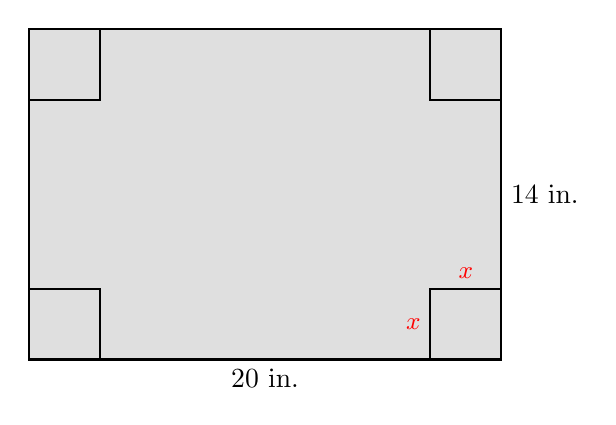
\begin{tikzpicture}[scale=0.3]
\fill[gray!25] (0,0) rectangle (20,14);
\draw[thick] (0,0) rectangle (20,14);
\foreach \a/\b in {0/0, 17/0, 0/11, 17/11} {\draw[thick] (\a,\b) rectangle ++(3,3);}
\node[below] at (10,0) {20 in.};
\node[right] at (20,7) {14 in.};
\node[above, red, font=\small] at (18.5,3) {$x$};
\node[left, red, font=\small] at (17,1.5) {$x$};
\end{tikzpicture}
\end{center}
\end{minipage}

\textbf{b.} Write and simplify a polynomial function $V$ to represent the volume of the tray. \\
{\small Volume $=$ length $\times$ width $\times$ height. Multiply two factors first, as in Example 2B.}

$V(x)=\blank[3.6cm]\cdot\blank[3.6cm]\cdot\blank[2cm]$
\lines[6]
$V(x)=\blank[1.5cm]\,x^3\;-\;\blank[1.5cm]\,x^2\;+\;\blank[1.5cm]\,x$

\newpage

\wspart{IXL}{Practice for the quiz}
Do the starred skills first. \textbf{SmartScore 70 or above on each starred ($\bigstar$) skill replaces your quiz score.}

\vspace{2pt}
\begin{tabularx}{\textwidth}{l Y Y}
\toprule
\textbf{Code} & \textbf{Skill} & \textbf{Feeds} \\
\midrule
\ixlrow{9A3 $\bigstar$}{Add and subtract polynomials}{Quiz 1 (add, standard form)}
\ixlrow{8GN $\bigstar$}{Multiply polynomials}{Quiz 2; Quiz 4 bonus (box)}
\ixlrow{DYB}{Polynomial vocabulary}{Warm-up: like terms, degree}
\bottomrule
\end{tabularx}

% DOK 3 kept: TE Practice & Problem Solving 13 (Reason, DOK 3, SEE EXAMPLE 1 in the item analysis). Key: 2, 1, or 0.
\wspart{Exit question}{Practice 13 (Reason)}
\fbox{\parbox{\dimexpr\textwidth-2\fboxsep-2\fboxrule}{%
Polynomial function $R$ is the difference of two degree-two polynomial functions. What are the possible degrees for $R$? Explain.

{\small Hint: subtract two degree-two polynomials whose $x^2$ terms have different coefficients, then two whose $x^2$ terms have the same coefficient.}
\lines[5]
The degree of $R$ can be \blank[3cm]. When I subtract, I combine \blank[2.4cm]. If the $x^2$ terms have the same \blank[2.4cm], they cancel, so the \blank[2cm] of $R$ goes down (when $R\neq0$; if every term cancels, $R=0$ has no degree).
}}

\vspace{6pt}
\textbf{Before the quiz, finish these sentences.}

Like terms have the same variables and the same \blank[3cm].

To subtract a polynomial, I distribute $-1$ to \blank[4cm] of its terms.

To multiply polynomials, I use the \blank[4cm] and then combine \blank[3cm].

A polynomial is in standard form when its terms go from highest to lowest \blank[3cm].

\end{document}
